%%%%%%%%%%%%%%%%%%%%%%%%%%%%%%%%%%%%%%%%%
% Large Colored Title Article
% LaTeX Template
% Version 1.1 (25/11/12)
%
% This template has been downloaded from:
% http://www.LaTeXTemplates.com
%
% Original author:
% Frits Wenneker (http://www.howtotex.com)
%
% License:
% CC BY-NC-SA 3.0 (http://creativecommons.org/licenses/by-nc-sa/3.0/)
%
%%%%%%%%%%%%%%%%%%%%%%%%%%%%%%%%%%%%%%%%%

%----------------------------------------------------------------------------------------
%	PACKAGES AND OTHER DOCUMENT CONFIGURATIONS
%----------------------------------------------------------------------------------------

\documentclass[DIV=calc, paper=a4, fontsize=12pt]{scrartcl}	 % A4 paper and 12pt font size

\usepackage{geometry}
\usepackage{multicol}
\usepackage{sectsty} % Enables custom section titles
\usepackage{minitoc}
%\usepackage{multicol} %Enables multiple columns and additional commands
\usepackage[utf8]{inputenc}
\usepackage[english]{babel} % English language/hyphenation
\usepackage[protrusion=true,expansion=true]{microtype} % Better typography
\usepackage{amsmath,amsfonts,amsthm} % Math packages
\usepackage[svgnames]{xcolor} % Enabling colors by their 'svgnames'
\usepackage[hang, small,labelfont=bf,up,textfont=it,up]{caption} % Custom captions under/above floats in tables or figures
\usepackage{booktabs} % Horizontal rules in tables
\usepackage{fix-cm}	 % Custom font sizes - used for the initial letter in the document
\usepackage{graphicx} %Use graphics and figures			
\usepackage{gensymb} %More symbols
\usepackage{float}
\usepackage{fixltx2e}
\usepackage[toc,page]{appendix}

\allsectionsfont{\usefont{OT1}{phv}{b}{n}} % Change the font of all section commands

\usepackage{fancyhdr} % Needed to define custom headers/footers
\pagestyle{fancy} % Enables the custom headers/footers
\usepackage{lastpage} % Used to determine the number of pages in the document (for "Page X of Total")

\usepackage{tcolorbox}

% Headers - all currently empty
\lhead{}
\chead{}
\rhead{}

% Footers
\lfoot{}
\cfoot{}
\rfoot{\footnotesize Page \thepage\ of \pageref{LastPage}} % "Page 1 of 2"

\renewcommand{\headrulewidth}{0.0pt} % No header rule
\renewcommand{\footrulewidth}{0.4pt} % Thin footer rule

\fancyfootoffset{0mm}

\usepackage{lettrine} % Package to accentuate the first letter of the text
\newcommand{\initial}[1]{ % Defines the command and style for the first letter
\lettrine[lines=2,lhang=0.3,nindent=0em]{
\color{DarkBlue}
{\textsf{#1}}}{}}

%----------------------------------------------------------------------------------------
%	TITLE SECTION
%----------------------------------------------------------------------------------------

\usepackage{titling} % Allows custom title configuration

\newcommand{\HorRule}{\color{DarkBlue} \rule{\linewidth}{1pt}} % Defines the gold horizontal rule around the title

\pretitle{\vspace{-30pt} \begin{flushleft} \HorRule \fontsize{22}{30} \usefont{OT1}{phv}{b}{n} \color{DarkBlue} \selectfont} % Horizontal rule before the title

\title{Biologisk skattejakt på planteten Mars \\ Prosessrapport \\ Gruppe 3} % Your article title

\posttitle{\par\end{flushleft}\vskip 0.5em} % Whitespace under the title

\preauthor{\begin{flushleft}\large \lineskip 0.5em \fontsize{12}{15} \usefont{OT1}{phv}{b}{sl} \color{DarkBlue}} % Author font configuration

\author{Ingelin Garmann, Simen L. Hegge, Karsten Olav Kjensmo, Jonas Sandøy Misund, Martin Nordal, Anna Solveig Julia Testani\`{e}re, } % Your name

\postauthor{\footnotesize \usefont{OT1}{phv}{m}{sl} \color{Black} % Configuration for the institution name
Norges Tekniske og Naturvitenskaplige Universitet % Your institution

\par\end{flushleft}\HorRule} % Horizontal rule after the title

\date{} % Add a date here if you would like one to appear underneath the title block

%----------------------------------------------------------------------------------------
%	SECTION TITLE
%----------------------------------------------------------------------------------------

\sectionfont{\Large \MakeUppercase}

\subsectionfont{\normalfont \MakeUppercase}

%----------------------------------------------------------------------------------------
%	TEXT
%----------------------------------------------------------------------------------------

\setlength{\columnsep}{32pt}
\linespread{1.2}

\geometry{
a4paper,
total={210mm,297mm},
left=15mm,
right=15mm,
top=20mm,
bottom=20mm}

%----------------------------------------------------------------------------------------
%	IMAGES
%----------------------------------------------------------------------------------------

\graphicspath{{Bilder/}}
\floatstyle{boxed}
\restylefloat{figure}

%----------------------------------------------------------------------------------------
%	APPENDIX
%----------------------------------------------------------------------------------------

\renewcommand\appendixpagename{Vedlegg}
\renewcommand\appendixtocname{Vedlegg}

%----------------------------------------------------------------------------------------

\begin{document}
\maketitle % Print the title

\thispagestyle{fancy} % Enabling the custom headers/footers for the first page 

%----------------------------------------------------------------------------------------
%	ABSTRACT
%----------------------------------------------------------------------------------------

% The first character should be within \initial{}

%----------------------------------------------------------------------------------------
%	ARTICLE CONTENTS
%----------------------------------------------------------------------------------------

\section*{Forord}

\begin{multicols}{2}


\end{multicols}

%----------------------------------------------------------------------------------------

\section*{Sammendrag}

\begin{multicols}{2}

\end{multicols}

%----------------------------------------------------------------------------------------

\pagebreak
\renewcommand{\contentsname}%
	{Innhold}

\tableofcontents

%----------------------------------------------------------------------------------------

\pagebreak
%\section{Innledning}

\section{Introduksjon til EiT}

Eksperter i team (EiT) er et obligatorisk emne for studenter som tar mastergrad på NTNU. 
Som forklart i emnebeskrivelsen\cite{eitlaeringsmaal} av faget, er hensikten med EiT å være et yrkesforberedende fag hvor studenten får erfaring med å arbeide i en tverrfaglig gruppe.
Emnet er utviklet på bakgrunn av at det i arbeidslivet ofte skal samarbeides i tverrfaglige prosjekter, en setting de færreste studenter har erfaring med før EiT.
Innsikt i gruppedynamikk skal læres ved å reflektere over og diskutere oppgaver, både innenfor et faglig prosjekt og en samarbeidsprosess.
Målet er at studentene skal bli bedre kjent med seg selv som en del av en gruppe, og hvordan gruppen og studenten påvirker hverandre.
Studenten skal utvikle sine samarbeidende egenskaper, bli komfortabel i å kommunisere, og lære hvordan å unngå samt håndtere konflikter.
Et like viktig mål med emnet er at studentene skal kunne formidle og anvende sin egen kunnskap og lære fra andres fagområder.
Læringsmålet innen samarbeid og læringsmålet innen tverrfaglig arbeid skal presenteres i to separate rapporter som vektes likt i det resulterende karakterresultatet.
\\

\begin{multicols}{2}

\end{multicols}

%----------------------------------------------------------------------------------------

\section{Landsbyen og gruppen}

\begin{multicols}{2}


\subsection{Landsbyen - Biologisk skattejakt på planeten Mars}

Landsbyen - Biologisk skattejakt på planeten Mars - består av rundt 20 medlemmer.
Disse er fordelt på tre grupper som hver for seg skal jobbe med de samme spørsmålene:
{\textit{Hva kan vi finne av liv/spor av liv på planeten Mars?
Hvordan kan dette fortelle oss mer om hvordan livet oppstod på vår egen planet?
Hva forteller dette oss om liv ellers i verdensrommet?}}















\subsection{Gruppemedlemmene}

For å gi et innblikk i hvilke medlemmer gruppen består av velger vi å presentere oss selv.
I de kommende avsnittene har vi alle skrevet om oss selv; hvem vi er, hvor vi kommer fra, hvilke interesser vi har og hvilke forventninger vi hadde til Eksperter i Team (både til fag og prosess).
\\

\subsubsection{Anna}

\paragraph{Personalia}
Er 25 år gammel, født og oppvokst i Sør-Frankrike. Jeg flyttet til Norge i 2007 og bodde også et år i Berkeley, California, i fjor.
Studerer teoretisk matematikk med fordypning i kryptografi. Masteroppgaven jeg skriver handler om elektroniske stemmesystemer.

\paragraph{Forventninger til EiT}
På forhånd hadde jeg hørt flest negative holdninger til EiT.
Dette var fra andre studenter som hadde hatt faget.
Likevel hadde jeg selv en positiv innstilling til faget siden jeg ikke hadde hatt gruppearbeid tidligere i utdanningen på NTNU.
Derfor var jeg nysgjerrig på hvordan det ville være.
Jeg syntes også at det hørtes lurerikt ut å reflektere rundt samarbeidet i seg selv.
Biologisk skattejakt på planeten Mars var mitt andrevalg som landsby på grunn av fasinasjonen for romfart.
Jeg var klar over at landsbyen lå utenfor mitt fagfelt og det var spennende med en utfordring!
\subsubsection{Ingelin Garmann}

\paragraph{Personalia}
23 år, oppvokst i Bergen og bodde der til utgangen av videregående med unntak av et skoleår på utveksling i Nevada, USA.
Gjennomførte et år med førstegangstjeneste i Hæren etter videregående.
Holder på med Siv.ing grad innen Industriell kjemi med spesialisering innen Kjemisk Prosessteknologi med størst interesse for prosesskontroll og reguleringsteknikk.
Driver med CrossFit og vektløfting på fritiden.

\paragraph{Forventninger til EiT}
Jeg var veldig spent på å arbeide i en tverrfaglig gruppe med stort fokus på selve gruppedynamikken.
Et slikt fokus er fremmed for de fleste innen tekniske studier, slik at jeg forventet og håpet å få god erfaring på området.
I tillegg til erfaring ønsket jeg å lære metoder for å unngå konflikter, og ikke minst bli mer bevisst på meg selv som person i en gruppe.
I tillegg var jeg spent på hvordan jeg kunne bidra faglig og hva jeg kunne lære av andre.
Landsbyen "Biologisk skattejakt på planeten Mars" var ikke ett av mine øverste valg da interessen for biologi ikke var så stor.
Jeg hadde forventninger om å kunne benytte både kreativitet og teknologi i en problemstilling som omhandlet kolonisering og terraforming av en planet.
På tross av at jeg hadde hørt negative bemerkninger om EiT, var jeg innstilt på å få noe positivt ut av faget!
\subsubsection{Jonas Sandøy Misund}

\paragraph{Personalia}
Jeg er født i Oslo i 1992 og oppvokst i Molde fra 1998.
Jeg studerer fysikk og matematikk med spesialisering innen teknisk fysikk ved NTNU.
Mye av fritiden min går med til frivillige verv, blant annet som hovmester i Lyche, restauranten på Studentersamfundet i Trondhjem.

\paragraph{Forventninger til EiT}
Eksperter i Team er et fag jeg har hørt både positive og negative ting om siden jeg begynte på NTNU.
Alt fra innslag under revyen, til venner som har vært læringsassistenter i fag har gitt meg inntrykk av EiT.
Selv hadde jeg ikke så mange tanker om hva vi skulle drive med i EiT, men ønsket å lære noe nyttig om gruppearbeid mens jeg deltok.
Gruppearbeid i seg selv er veldig interessant og moro å drive med, så jeg gledet meg litt til å få noe mer håndfast kunnskap om nettopp dette.
Ellers er jeg, som den fysikknerden jeg er, ganske interessert i omtrent alt som foregår ute i verdensrommet.
Mars er jo nettopp noe som \textit{foregår} ute i verdensrommet.
Derfor ble "Biologisk skattejakt på planeten Mars" en av landsbyene jeg satte opp som alternativer.
\subsection{Karsten Olav Kjensmo}

\paragraph{Personalia}
25 år. Har vokst opp i bl. a. Danmark, Nigeria, Namibia og USA. Opprinnelig født i Bærum, men har har ikke gått på norsk skole eller bodd lenge i Norge før universitetstiden. Har gjennomført en bachelorgrad i informatikk, og går mastergrad i informatikk på linjen databaser og søk; hvor jeg skriver oppgave innen kunstig intelligens og webteknologi. Har derutover faglig interesse i kognitive arkitekturer og designteori knyttet til menneske-maskin interakjson. På fritiden sykler jeg på fjellet, driver med hobbybryting og knoter med datateknologi. 

\paragraph{Forventninger til EiT}
Ved fagets start var inntrykket godt. En god studiekamerat har tatt både faget og den spesifikke landsbyen før, og hadde bare gode ting og si. Det ble kommentert på den trivelige stemningen i landsbyen - noe som alle landsbyer ikke har - samt den faglige friheten knyttet til oppgaven og emnet. Det faglige trakk av flere grunner - jeg er amatør på biologifeltet, men mente ikke dette ville være et problem, da jeg trodde det ville være mange biologer på landsbyen og at jeg med datavitenskap ville kunne bringe en ny vinkel på deres felt, spesifikt med datavitenskapen knyttet til romfart og utforskningsroboter. Det sosiale var også en faktor, da det ikke er mangel på skrekkhistorier om EiT grupper (nok noe overdrevet eller selvpåført) som ikke hang sammen sosialt. Andre studiekamerater har kommentert på dette, og har mistrivdes stort, og dette var et element i avgjørelsen da jeg valgte å søke landsbyen for biologisk skattejakt på Mars. Ved fagets start var jeg altså innstillt på å lære fra andre fagfelter, samt teste meg selv i en sosial arena med et introspektivt fokus. 





\subsubsubsection*{Martin Nordal}

\paragraph{Personalia}
Er 24 år og kommer fra Oslo.
Interessen for programmering og skripting fikk meg til datateknikk-studiet, etterhvert med retning kunstig intelligens.
Har også interesse for romfart, noe som førte til at jeg søkte på denne EiT-landsbyen.

\paragraph{Forventninger til EiT}
Forhåndsinntrykket til EiT har til dels vært basert på beretninger fra eldre personer som har hatt faget tidligere.
Det gjentakende i deres beretninger har vært at faget inneholder for mye obligatoriske aktiviteter som ikke har vært oppfatta som nyttig, mens det ble altfor liten tid til å arbeide med eventuelle prosjekter eller de endelige rapportene.
Gjennom studiene så langt har jeg selv vært med på mye gruppearbeid.
Det har stort sett vært trivelig og produktivt, men enkelte gruppesammensetninger, og kanskje spesielt de store gruppene, ikke har fungert så bra.
EiT kunne derfor være behjelpelig for å lære hvordan man i fellesskap skal takle menneskelige utfordringer i en gruppe.
\subsubsection{Simen Løvøy Hegge}

\paragraph{Personalia}
Jeg er 23 år gammel og kommer fra Kunes, en liten plass midt i Finnmark med 30 innbyggere.
Bor for tiden i Trondheim sammen med min samboer og vår sønn på snart to år.
Vi venter vårt andre barn høsten 2015.
Jeg har en bachelorgrad innen allmenn bygg fra Høgskolen i Narvik, og bygger nå på med 2-årig master på bygg og miljøteknikk, retning konstruksjon ved NTNU.

\paragraph{Forventninger til EiT}
Høgskolen i Narvik hadde ingen fag som het (eller minnet om) EiT.
Jeg hadde derfor aldri hørt om faget før jeg begynte på NTNU.
Hørte fa en del negative ting om faget fra medelever her på NTNU, men lot ikke dette påvirke mitt inntrykk. 
Det hørtes ut som et nyttig fag med tanke på samarbeid.

Denne landsbyen var ikke førstevalget siden den ikke treffer fagfeltet mitt.
Ordet "biologi" føles langt fra fagfeltet konstruksjon, men utforsking av Mars pirret romfartsinteressen min.
Denne landsbyen ble derfor andrevalget.

\end{multicols}

%----------------------------------------------------------------------------------------

\section{Metodebeskrivelse}

\begin{multicols}{2}

\subsection{Rammeverk}

Landsbyen "Biologisk skattejakt på planeten Mars" er en langsgående landsby.
Det innebærer obligatorisk oppmøte hver onsdag i 15 uker. Før de resulterende rapportene fra prosjekt- og prosessoppgaven kan leveres, må gruppen holde en muntlig prosjektpresentasjon og delta på en prosessamtale med læringsassistenter og landsbyleder.
De to rapportene har innleveringsfrist en uke etter siste landsbydag. Begge rapportene teller like mye på en felles karakter for gruppen.
\input{"Metodebeskrivelse/Innsjekk_reflektering_utsjekk"}

\end{multicols}

%----------------------------------------------------------------------------------------

\section{Generell teori}

\begin{multicols}{2}

\end{multicols}

%----------------------------------------------------------------------------------------

\section{Gruppeutvikling}

\begin{multicols}{2}
\input{"Gruppeutvikling/Gruppeutvikling_intro"}

\input{"Gruppeutvikling/kommunikasjon/kommunikasjon_intro"}
\input{"Gruppeutvikling/effektivitet/effektivitet"}
%\input{"Gruppeutvikling/konflikt/konflikt_main"}
\input{"Gruppeutvikling/konflikt/konflikt_intro.tex"}
\subsubsection{Konfliktdefinisjon}

\paragraph{Begrepsforståelse}
\emph{Konflikt} er et ord som kan dekke alt fra en uenighet om hvor mye sukker som skal i kaffen, til moderne krig i stor skala. Konflikt tildeles muligvis en mere aggressiv og intens betydning i folketale, men i EiT rammeværket vil vi være gankse presise i vår forståelse av begrepet. Vi mener det er en forskjell mellom uenighet og konflikt, og at de ligger en følelsesladet forskjell mellom en redelig debatt og en kamplignende konflikt. Saklig uenighet bidrar til nytenkning og fremdrift, mens konflikt fører til stagnasjon, nedsatt produktivitet og mistrivsel\cite{ledernytt}. Partene i en konflikt går i hver sine skyttergraver, og det blir slutt på utforskning, dialog og konstruktivt samarbeid. I denne seksjonen vil vi henvise oss til faglitteraturen innen ledelse og administrasjon, og undersøke årsaker som bidrar til konflikter på gruppen. Dette vil stille gruppens konfliktsituasjon i et klarere lys. 


\paragraph{Hvorfor går det galt?}




Liste av årsaker til konfliktfyllte grupper\cite[p.~253]{orgorg}

\begin{itemize}

  \item Gruppemedlemmene tar stilling og nekter å gå inn på kompromiss.
  \item Gruppemedlemmene viser utålmodighet overfor hverandre.  
  \item Ideer blir angrepet før de er blitt ferdig fremlagt.
  \item Gruppemedlemmene angriper hverandre personlig.
  \item Gruppemedlemmene anklager hverandre for ikke å forstå hva som er viktig.
  \item Gruppemedlemmene oppfatter bare fragmenter av det de andre sier.  

\ldots
\end{itemize}
\subsubsection{Positiv innstilling til faget}

Fra begynnelsen av prossessen har hvert enkelt medlem av gruppen vært positivt innstilt og dedikert, noe som gjorde at en hel avdeling av potensielle konflikter ikke oppstod.
\\
Gruppen har ikke opplevd motstand om faget fra enkelte individ, hverken på prosjekt- eller prosessdelen. 
Medlemmene hadde like forventninger til faget. Uansett hvor ukomfortabelt eller vanskelig det var å skrive personlig refleksjon i den første fasen, gjorde gruppen en god innsats og prøvde å få noe ut av det.
Denne innstillingen rettet mot fagets øvelser og rammeverk som helhet, og at slike typer oppgaver ble tatt seriøst med en gang, bidro til at gruppen unngikk noen form for motivasjonskonflikt.
\\
Gruppen ble oppmerksom allerede da kompetanstrekanten ble laget, at ingen hadde ekspertise innenfor hverken biologi (prosjekt) eller humaniora (prosess).
Dette gjorde at gruppen ble bekymret for å stille ganske svakt på faglig kunnskap innenfor landsbyens hovedtema.
Gruppen har i etterkant forstått at dette har også hjulpet i samarbeidet, da alle har startet fra samme sted rent faglig.
Dette gjorde at det ikke ble noe faglig dominans fra et individ, noe som kunne ha skapt konflikt eller forstyrret balansen i arbeidsfordelingen.
Som konsekvens av dette var medlemene ydmyke, åpen for forskjellige løsninger, og alle fikk mulighet til å bidra likt på oppgavene.
Det som var sett som en svakhet i begynnelsen ble en av grunnene til mangelen på større konflikter.
\\
Gruppen har også gjort en god jobb rundt konfliktprevensjon i oppstartsfasen. 
Medlemmene satte struktur og regler med virkemidler som arbeidskontrakten og individuelle mål. 
Medlemmene har vist respekt for målet til EiT og har vært flinke til å definere oppgaver, ansvar og mål.
Gruppen ble for eksempel enig om å ha som mål å jobbe mot en A; formuleringen i arbeidskontrakten er at alle skal levere en \emph{innsats} tilstrekkelig for toppkarakter.
At forventninger til både faget og hverandre ble avklart tidlig gjorde at konflikt rundt selve strukturen ikke har oppstått. Gruppemedlemmene kunne ikke anklage hverandre for ikke å forstå oppgavene eller målet.
Det har aldri vært et problem å møte utenom onsdager, til privat jobbing der dette trengtes.
Inkluderende medlemmer og et positivt forhold til faget gjorde at deltagerne følte eierskap og ansvar i samarbeidet.
Alle medlemmene ble inkludert og ingen fikk mulighet til å melde seg ut.
Som konsekvens av disse faktorene har gruppen ikke hatt noen interessekonflikter.
\\
\subsubsection{Gruppens sosiale interaksjon}

Hovedtemaet i denne seksjonen er å undersøke det sosiale samværet, samt diskutere hvilke effekter dette har hatt på gruppen.
Her vil gruppen støtte seg til faglitteratur\cite{orgorg}, og se på forhold som særpreger effektive grupper. 
Busch, Vanebo og Dehlin\cite[p.~257]{orgorg} lister opp en rekke sosiale kvaliteter som markerer et godt samarbeid: åpen kommunikasjon, gjensidig tillit, sosial støtte, og utnyttelse av individuelle forskjeller.
Disse vil behandles i lys av EiT prosessen.
I følgende tekst skal det positive og det negative i hver kategori undersøkes.
En gjennomgående faktor i alle kategoriene er gruppens innstilling til EiT. 
Alle de følgende punktene kan kommenteres i lys av gruppens sosiale utvikling. 
Samarbeidsindikatorene er presentert i kapitellet om kommunikasjon, men for tydelighets skyld gjentas de her, da de nå skal behandles fra konfliktperspektiv. 

\begin{figure}[h!]
  \caption{Samarbeidsindikator 1, tidlig i faget}
  \centering
    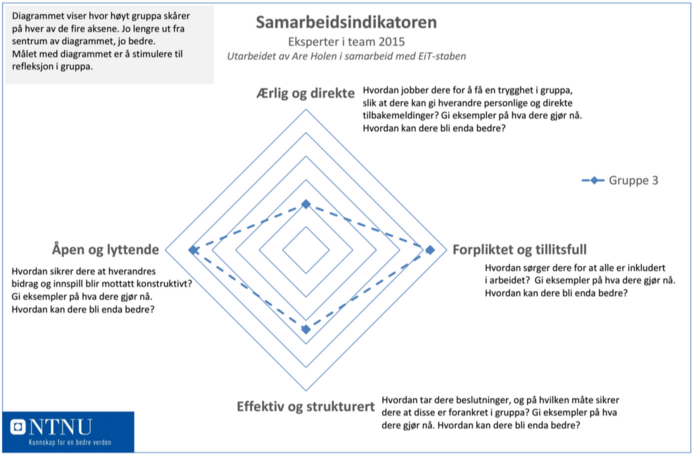
\includegraphics[width=0.5\textwidth]{Bilder/samarbeidsindikator1.png}\label{samarbeidsindikator1}

\end{figure}
\begin{figure}[h!]
  \caption{Samarbeidsindikator 2, midt i faget}
  \centering
    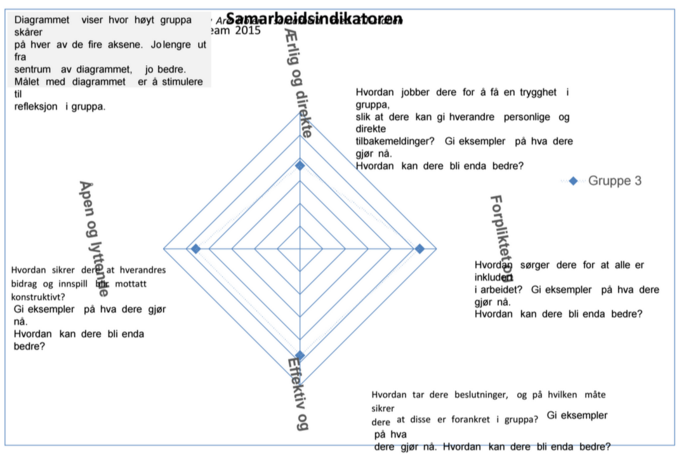
\includegraphics[width=0.5\textwidth]{Bilder/samarbeidsindikator_2.png}\label{samarbeidsindikator2}
\end{figure}

\begin{figure}[h!]
  \caption{Samarbeidsindikator 3, mot slutten av faget}
  \centering
    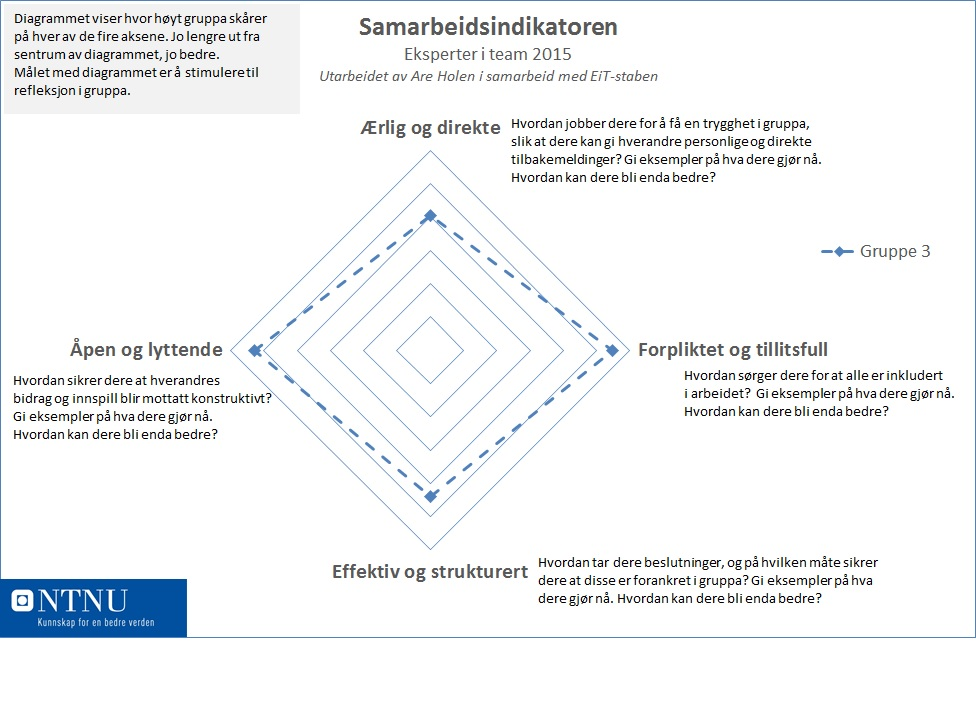
\includegraphics[width=0.5\textwidth]{Bilder/samarbeidsindikator_3.jpg}\label{samarbeidsindikator3}
\end{figure}

\emph{Åpen kommunikasjon} har gruppen hatt bra utslag på ifølge undersøkelsene siden starten av faget. 
Dette er noe gruppen har gjort bra, med unntak av oppstartsfasen (se figur \ref{samarbeidsindikator1}).
Her er det snakk om gruppens sentimenter omkring ærlig og direkte oppførsel, hvor resultatet var lavt.
Denne dualiteten var noe gruppen stusset over - det var overraskende at resultatet på ærlighet var så lavt, og dette gjorde inntrykk ved at det ble tatt opp gjentagne ganger da resultatene var klare.
Resultatet for 'åpen og lyttende' atmosfære har vært vedvarende høy, og 'ærlig og direkte' gikk mot høyere resultat (se figurer \ref{samarbeidsindikator2}, \ref{samarbeidsindikator3}).
Gruppen reflekterte over dette, og kom frem til at det hersker en spesiell atmosfære når en gruppe er ny, og medlemmene vet at de skal samarbeide i lang tid.
Her vil det ofte være ivrighet til å skape en god stemning; folk vil le høyere av vitser som de ikke synes er så morsomme, de vil være mer tålmodige med andres bagateller, og være ekstra følsom for å levere en negativ tilbakemelding.
Gruppemedlemmene skjønner at ærlighet ofte holdes skjult under en fasade av høflighet, men skjønner også at dette gjøres for å sikre en trygg og samtalevennlig atmosfære. Det tok noen landsbydager før gruppen kunne behandle hverandes væremåte ærlig.
Et spesifikt eksempel er at Anna ventet til landsbydag fire med å kommentere at Jonas hadde en tendens til å snakke for mye, hvor det ble behandlet med rolig gemytt. 
Som kommentert på tidligere i rapporten, kan en gruppes sosiale samvær justeres etter hvert når medlemmene er mere komfortable med hverandre. 
Gruppen mener at den tidlige stemning var velment, men hindret ærlig og direkte kommunikasjon tidlig i prosessen, slik som samarbeidsindikatoren viser. 
Dette kunne da også ha bidratt til den trivelige sosiale atmosfæren; kanskje en startfase hvor ubehageligheter pakkes godt inn i diplomatiske utsagn er noe som skal til for å danne et trygt grunnlag.
Som samarbeidsindikatoren viser, gled gruppen inn i en meget trygg sosial atmosfære, som siden har vært en svært positiv innflytelse på gruppens samarbeid.\\
\\
\emph{Gjensidig tillit} må opparbeides. 
Det er få situasjoner hvor folk som er fremmed for hverandre og hverandres bakgrunn føler seg komfortable før interaksjon.
Tilliten i gruppen har kommet av en universell motivasjon for å jobbe sammen. 
I oppgavene i de første ukene demonstrerte gruppen viljen til å  arbeide og samarbeide.
Med en åpen og lyttende natur hvor det har vært ønsket at alle skal bli hørt, har dette ført til en atmosfære av gjensidig tillit. 
Selv når folk har kommet for sent, eller levert arbeid for sent, har det ikke vært foruroligende grunnet den underliggende tilliten.
Her kan vi også observere at en økt gjensidig tillit kan føre til at medlemmene er litt mer avslappet rundt tidsfrister.
Skulle det være fremmede eller sterkt kritiske kollegaer ville det være større grunn til sosial stress.
Dette ville da kanskje føre til at medlemmene var mere stringent med tanke på frister, men ville skape større sjanse for en potensielt destruktiv konfrontasjon.\\
\\
\emph{Sosial støtte} vokste frem stille og rolig, drevet mye av et økt sosialt velbehag, samt innsjekk og utsjekk. 
De faglig rammene for hver landsydag var grobunn for innsikt i hverandres liv. 
Derfor ble innsjekk og utsjekk alltid tatt på alvor. 
I disse 'øyeblikk' har individer fått mulighet til å vise tillit til hverandre og inkludere resten av gruppen i livet sitt. Referatene viser til en trend i å dele 'historier'; gruppen har fulgt Ingelins kvalifisering til NM i vektløftning, Simens fortellinger om sin sønn, Annas beslutning tidlig i prosessen til røykestopp og maratonløping, og Jonas sitt ansvar som hovmester på Samfundet er noen eksempler vi kan ta som viser til dette punktet.
En god sosial kommunikasjon og en trivelig tone har skapt et positivt og trygt arbeidsmiljø\cite{happy}.
Medlemmer får lyst å samarbeide og føler seg mer komfortable, hvis de føler seg verdsatt som mere enn bare et verktøy i et fag.\\
\\
\emph{Utnyttelse av individuelle forskjeller} på sosialt plan er noe annet en på et faglig plan.
Et godt sosialt miljø gjorde at medlemmene ble klar over hvilke personlighetstyper som finnes i gruppen.
Dette er informasjon som er \emph{svært viktig} i et samarbeid.
Fra begynnelsen av prosessen har hvert enkelt medlem i gruppen vært inkluderende og dedikerte til laginnsatsen. 
Dette har gjort det mye lettere å bli kjent med hverandre.
De forskjellige personlighetstypene har påvirket gruppen på hver sin måte.
I gruppen har dette vist seg ved at Jonas og Karsten har oppført seg som verv-erfarne initiativtakere,  Martin og Simen har formidlet gjennomtenkte og reflekterte utsagn, og Anna og Ingelin har hatt nøye blikk for struktur og fremdrift.
Gruppen hadde også en overordnet tendens til å fremheve den positive siden over den negative siden.
Annas usikkerheter rundt det norske språket har ikke vært til bry for gruppen, og hun føler seg tålmodig behandlet.
På samme måte \emph{kunne} det vært sett på som en negativ ting at Jonas ofte fører ordet, men gruppen la heller merke til hvor mye han bidro.
Gruppen har altså ikke latt seg irritere over ting de ikke kunne gjøre noe med, og heller vært adaptive og fokusert på fordeler og styrker.
\\
\subsubsection{Konfliktskyhet}

\paragraph{Konflikter i gruppesituasjonen}
Konfliktskyhet er en naturlig egenskap å ha, spesielt i kulturen som hersker i det moderne Norge.
Konflikter er ubehagelige, stressende, krever store mengder energi og resulterer ofte i mellommenneskelig skade.
Forhold som har vært gode kan bli dårlige og forhold som har vært dårlige kan bli helt ødelagt.
Det er alltid noe på spill utover det diskuterte når en konflikt skjer, og spesielt i gruppeatmosfærer kan en enkelt konflikt ha varige skader lenge etter konflikten fant sted. 
En konflikt kan bygges opp sakte eller skje spontant, og konfliktskyhet fremkommer i begge tilfeller. 
De fleste velger konfliktene sine med omhu. Noen ganger må en konfrontasjon finne sted for at man skal føle seg respektert, eller for å behandle en situasjon som oppfattes som er urettferdig. 
Noen situasjoner er ikke verd de potensielle negative følger, og folk finner derfor andre måter og forholde seg til konflikten på. 
\\
\paragraph{Konflikter i gode sosiale miljø}
Dette kan man observere i EiT, hvor konfliktskyhet kan ha mange årsaker, og resultere i mange forskjellige utfall.
Den gode sosiale tonen innad i gruppen kan ha vært en barriere for direkte kommunikasjon - noe som kommenteres på i forbindelse med den første samarbeidsindikatoren som finnes på side \pageref{samarbeidsindikator1}. 
Her er scoren for gruppens evne til å være ærlig og direkte var meget lav.
Dette endret seg over tid, men er allikevel indikativt på at overdiplomatiske ordvalg har begrenset kommunikasjon.
Det var, tidlig i prosjektet, en stor frykt for å skape unødvendig dårlig sosial trivsel. 
Kan gruppen ha blitt enda mer konfliktsky av den gradvis økende sosiale atmosfæren, eller har dette gjort det enklere å snakke direkte?
Gruppen har lurt på om frykten for sosial friksjon har vedvart, eller om den har blitt gradvis mitigert av et styrket sosialt bånd.
Dette viser samarbeidsindikator 2 og 3 viser til, men det kan fortsatt være en blanding av faktorene. 
\\
\paragraph{Tid som hjelpende faktor}
Det gikk en uke mellom hver landsbydag, og en uke er god tid til å fordøye inntrykk, tenke over saker og la emosjoner falle til ro. 
Til sammenligning med EiT intensiv, hvor arbeidet foregår over meget kort tid, er en ukes pusterom mellom hver hele landsbydag god tid til å fatte ro.
Gruppen mener det har hatt en positiv effekt på konflikthåndteringen. 
Det har skjedd flere ganger at et medlem har gått fra landsbydagen med et negativt inntrykk av en situasjon, hvor angrep og forsvar har blitt vekslet jevnt, og at dette negative inntrykket reduseres når medlemmet får tid til ro.
Ved neste ukes møte er den negative situasjonen behandlet, og begge parter er roligere og vennligere innstilt.
Et eksempel på dette er en interaksjon mellom Ingelin og Karsten.
Etter prosjektskrivingens start hadde Ingelin gjort noen spøkefulle kommentarer om Karstens skrivemåte.
Dette tok Karsten først til hjertet som mobbing, men etter en uke til å la inntrykket fordøye seg skjønte han at det slettes ikke var vondt ment.
Det viste heller til en grad av sosial komfort, som gjorde at Ingelin turte å spøke med Karsten uten frykt for negative konsekvenser. 
\\
\paragraph{Innordning vs. underkastelse}
En av de meste effektive våpnene i konfliktprevensjon er å være komfortabel med å innordne seg når situasjonen nå krever det. 
Det er en forskjell mellom innordning og underkastelse. 
Ved underkastelse forstås en mishandling: et medlem føler seg såpass presset og urespektert at en sterk og legitim mening blir holdt tilbake. 
Underkastelse er skadelig, og tilsier at det er virkemidler på spill som ikke baserer seg på rolig og resonnerende debatt.
Ved innordning forstås en diplomatisk handling: den innordnende har presentert sine argumenter og disse overbeviser ikke.
Den innordnede har forstått at h*n er i mindretall og at en fortsettelse av debatten ikke vil tjene noe godt formål.
Den innordnede har altså gode følere for både hvor viktig diskusjonen er, og for resten av gruppens holdning til diskusjonen.
Det har hersket mye diskusjon i gruppen, som i generelle trekk har valgt å fremgå mere metodisk og grundig i alle avgjørelser.
Ved å diskutere jevnlig, har enkelte medlemmer vært nødt til å innordne seg flertallets meninger. 
Et eksempel på dette er Karstens tidlige forslag om å bruke programmet Trello til arbeidsplanlegging. 
Dette verktøyet brukes ofte på informatikkstudiet og Karsten argumenterte for at det ville være en god id\'{e} å bruke. 
Resten av gruppen ble ikke overbevist, og da det allerede skulle brukes en del verktøy som var nye for gruppen ble dette forslaget nedstemt. 
Karsten innordnet seg etter nedstemmingen og argumenterte ikke videre for bruk av Trello. 
\\
\paragraph{Preventiv vs. reaktiv konfliktshåndtering}
Konfliktløsning er en av de sentrale konseptene i EiT.
Mangeler på større konflikter i gruppen har vært en bekymring for fagets læringsmål og for karakteren. 
Faglig skulle det helst ha forekommet en større konflikt eller to, slik at gruppens medlemmer fikk prøvd seg på reaktiv konfliktløsning. 
Ved å forholde seg diplomatisk midt i en ubehagelig gruppesituasjon og teste ut virkemidlene beskrevet forskjellige steder i pensum. 
Dette fikk gruppen ikke gjort på stor skala.
Derimot har det blitt demonstrert kapasitet for prevantivt konfliktshåndtering. 
Konflikter har blitt behandlet før de fikk utartet seg til noe større. 
Gruppens samarbeid har vært rettet mot en preventiv holdning, og denne kan sies å ha utspillet seg med suksess. 
Her kan det vises til grunnreglene for effektive grupper\cite{schwarz}, spesifikt regel fem. 
Når et fellesskap skal komme til enighet hender det at noen er tidlig ute med et forslag til løsning.
Da stiller vedkommende seg i en posisjon hvor det er ukjent for de andre hvilke interesser denne personen legger til  grunn for en slik løsning, og stien til målet kan være uklar. 
Hvis stien til målet er uklar, kan det skape forvirring i resten av grupppen. 
Slike forslag og motforslag kan nemlig være inkompatible selv om interessene egentlig stemmer overens.
Hvis man åpner med å dele interesser med de andre, er det lettere å utarbeide løsninger i fellesskap.
Ved diskusjoner rundt rapportens utforming, for eksempel, gjorde medlemmene mye ut av å presentere den større visjonen de forestilte seg før de gikk inn på detaljene om hvordan denne visjonen skulle nåes. 
Om andre tidlig kommer med løsninger istedet for å begrunne dem, kan man spørre om interessene som ligger til grunn.
\\
\subsubsection{Undergrupper}

Gruppen ville undersøke om det hadde formet seg noen undergrupper/klikker underveis i arbeidet, og om disse kunne ha innflytelse på arbeidet.
Ved starten var det ingen som kjente til hverandre, så det ble en egalitær start.
Dette ble bygget videre på med en inkluderende gruppekultur. Det ble også lagt mye fokus på at alle skulle få sagt det de ville i innsjekk- og utsjekksrutinen. 
Disse faktorene har medført mindre muligheter for undergrupper. 
Det vil ikke kunne sies at det ble dannet undergrupper. 
Enkelte gruppemedlemmer interagerte bedre med hverandre enn andre, for eksempel Karsten og Martin som både har felles fagbakgrunn og skolevei ble godt sammensveiset. Anna og Ingelin hadde lignende arbeidsstil og jobbet mer sammen i par enn andre. 
Det kan spørres om gruppen hadde dannet klikker og undergrupper om prosjektet hadde foregått over enda lengere tid.
Var dette en toårskontrakt og ikke et semesterfag, ville det kanskje ha oppstått sterkere kliker som kunne ha påvirket arbeidet. 


\subsection{Kompetansetrekant}

Allerede andre landsbydag fikk gruppen i oppgave å lage en kompetansetrekant. Kompetansen ble evaluert innenfor tre kategorier: teoretisk kunnskap innenfor sitt fagfelt, praktisk erfaring og personlige trekk. 
I første omgang laget hvert medlem en individuell trekant, for så å presentere sine evner til gruppen. 
Til slutt samarbeidet gruppen om å lage en trekant som representerte hele gruppens kompetanse.
Hensikten med oppgaven var å bevisstgjøre gruppemedlemmene om sin individuelle kompetanse og gi innsikt i de andre medlemmenes kompetanse. 
På dette tidlige tidspunktet kjente ikke gruppen til hver enkelts kompetanse og var heller ikke vant til å evaluere sine egne kunnskaper.

Det mest slående med gruppens endelige kompetansetrekant var spredningen i fagfelt.
En heterogen gruppe er ofte en fordel.
Personer med ulik bakgrunn vil ha ulike løsninger, tanker og ideer om samme problemstilling. 
På denne måten oppnår man et høyere nivå av forståelse, blir introdusert for nye innsynsvinkler og kan besvare problemstillingen grundigere.
Mangfoldet gir grunnlag for en dynamisk diskusjon der et individs opprinnelige ide vil bli utviklet videre av hele gruppen.
Resultatet er at ideen får et forbedret og bredere innhold enn det et enkeltmedlem alene har kompetanse til å besvare.
Et slikt samarbeid krever at medlemmene klarer å formidle sine ideer til fellesskapet.
Når gruppen er heterogen er det viktig at ideer blir formidlet slik at alle forstår budskapet.
Like viktig som å være en god formidler, er det å kunne lytte til andres ideer. 

Den og mangelen på kunnskap innen biokjemi.


\end{multicols}

%----------------------------------------------------------------------------------------

\section{Konklusjon}

\begin{multicols}{2}

\subsection{Hva har gruppemedlemmene lært?}

\subsection{Hva har gruppen lært?}

\subsection{Læringsmål}

\end{multicols}


%----------------------------------------------------------------------------------------
%	REFERENCE LIST
%----------------------------------------------------------------------------------------

\onecolumn
\small{
\input{"Kilder.tex"}
}

%----------------------------------------------------------------------------------------
%	APPENDIX
%----------------------------------------------------------------------------------------

\pagebreak

\begin{appendices}
\section{Samarbeidsavtale}
\label{Ved:samarbeidsavtale}
\begin{center}	
	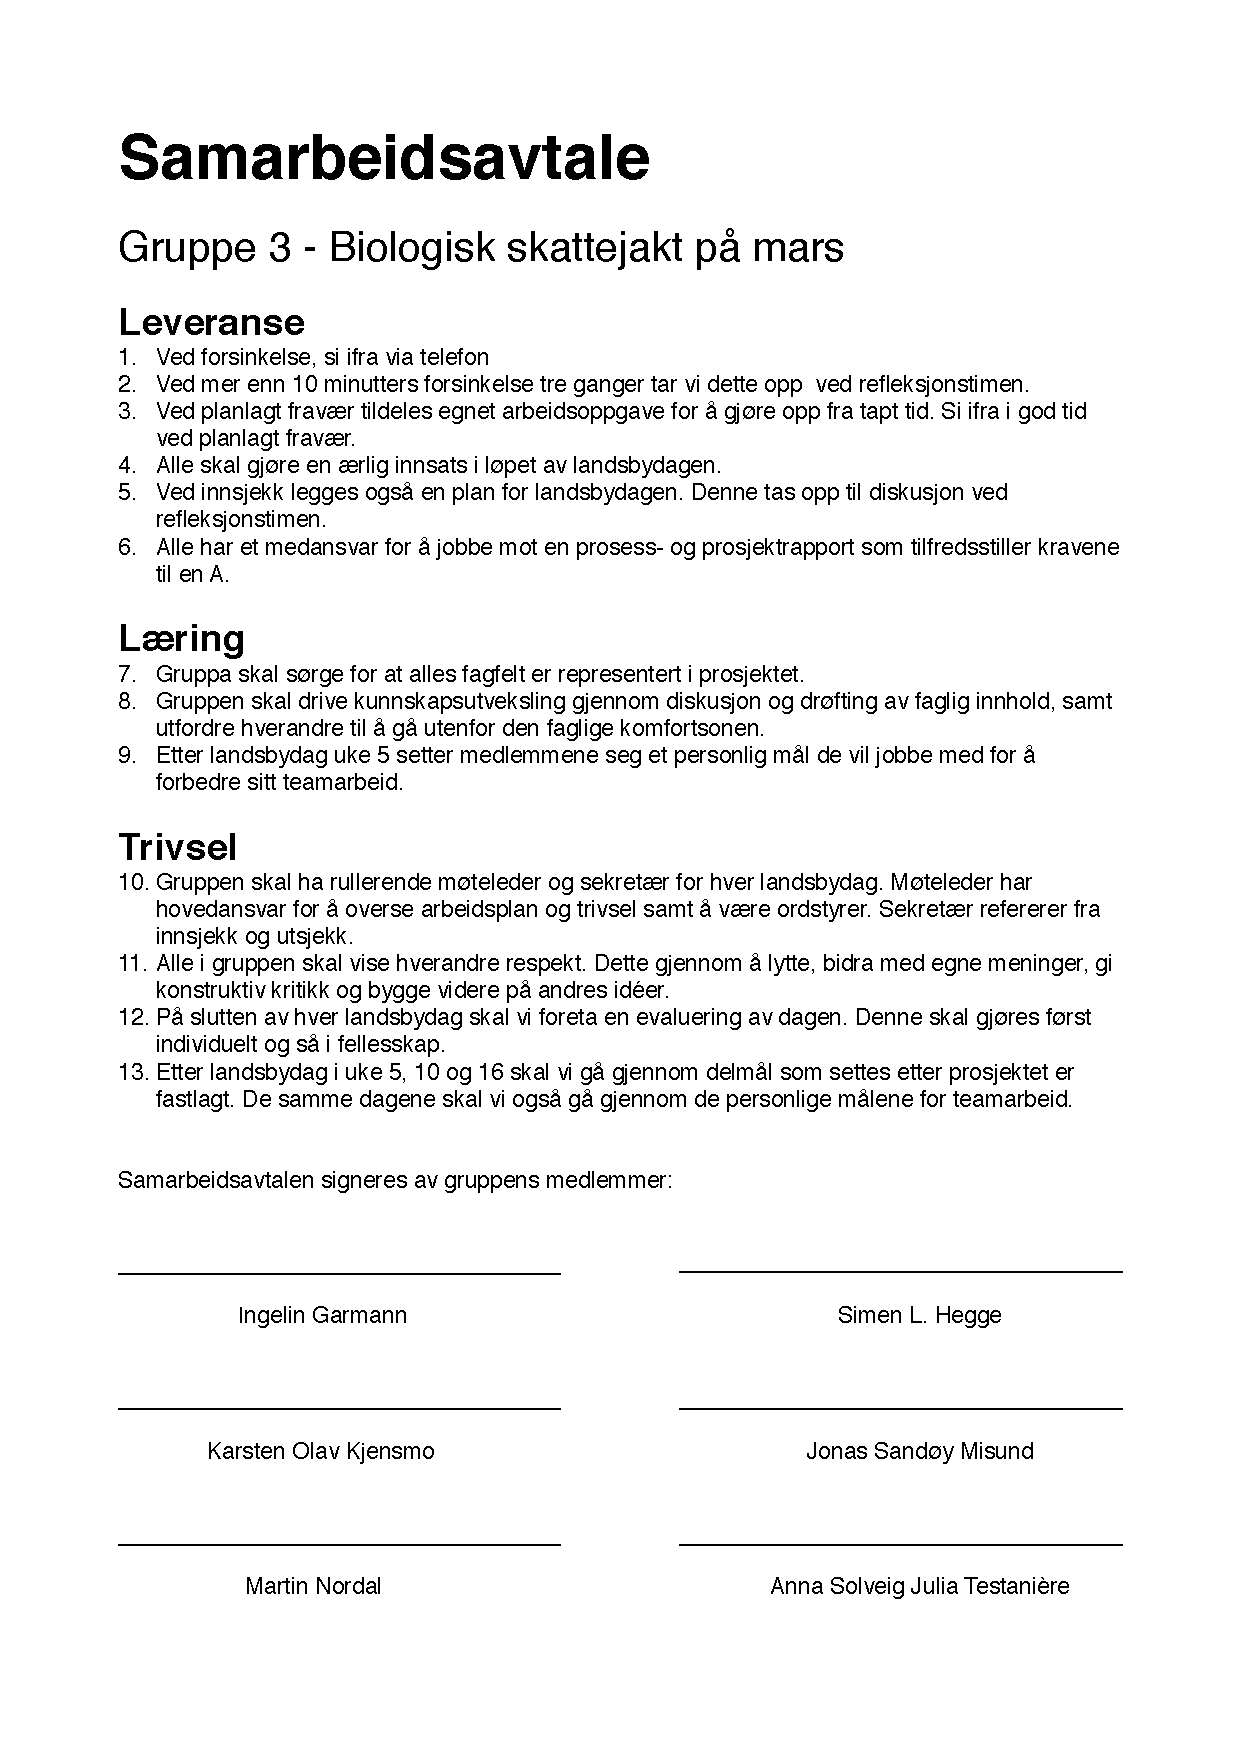
\includegraphics[width=0.9\textwidth]{Samarbeidsavtale.pdf}
\end{center}

\section{Samarbeidsavtale versjon 2}
\label{Ved:samarbeidsavtale_2}
\begin{center}
	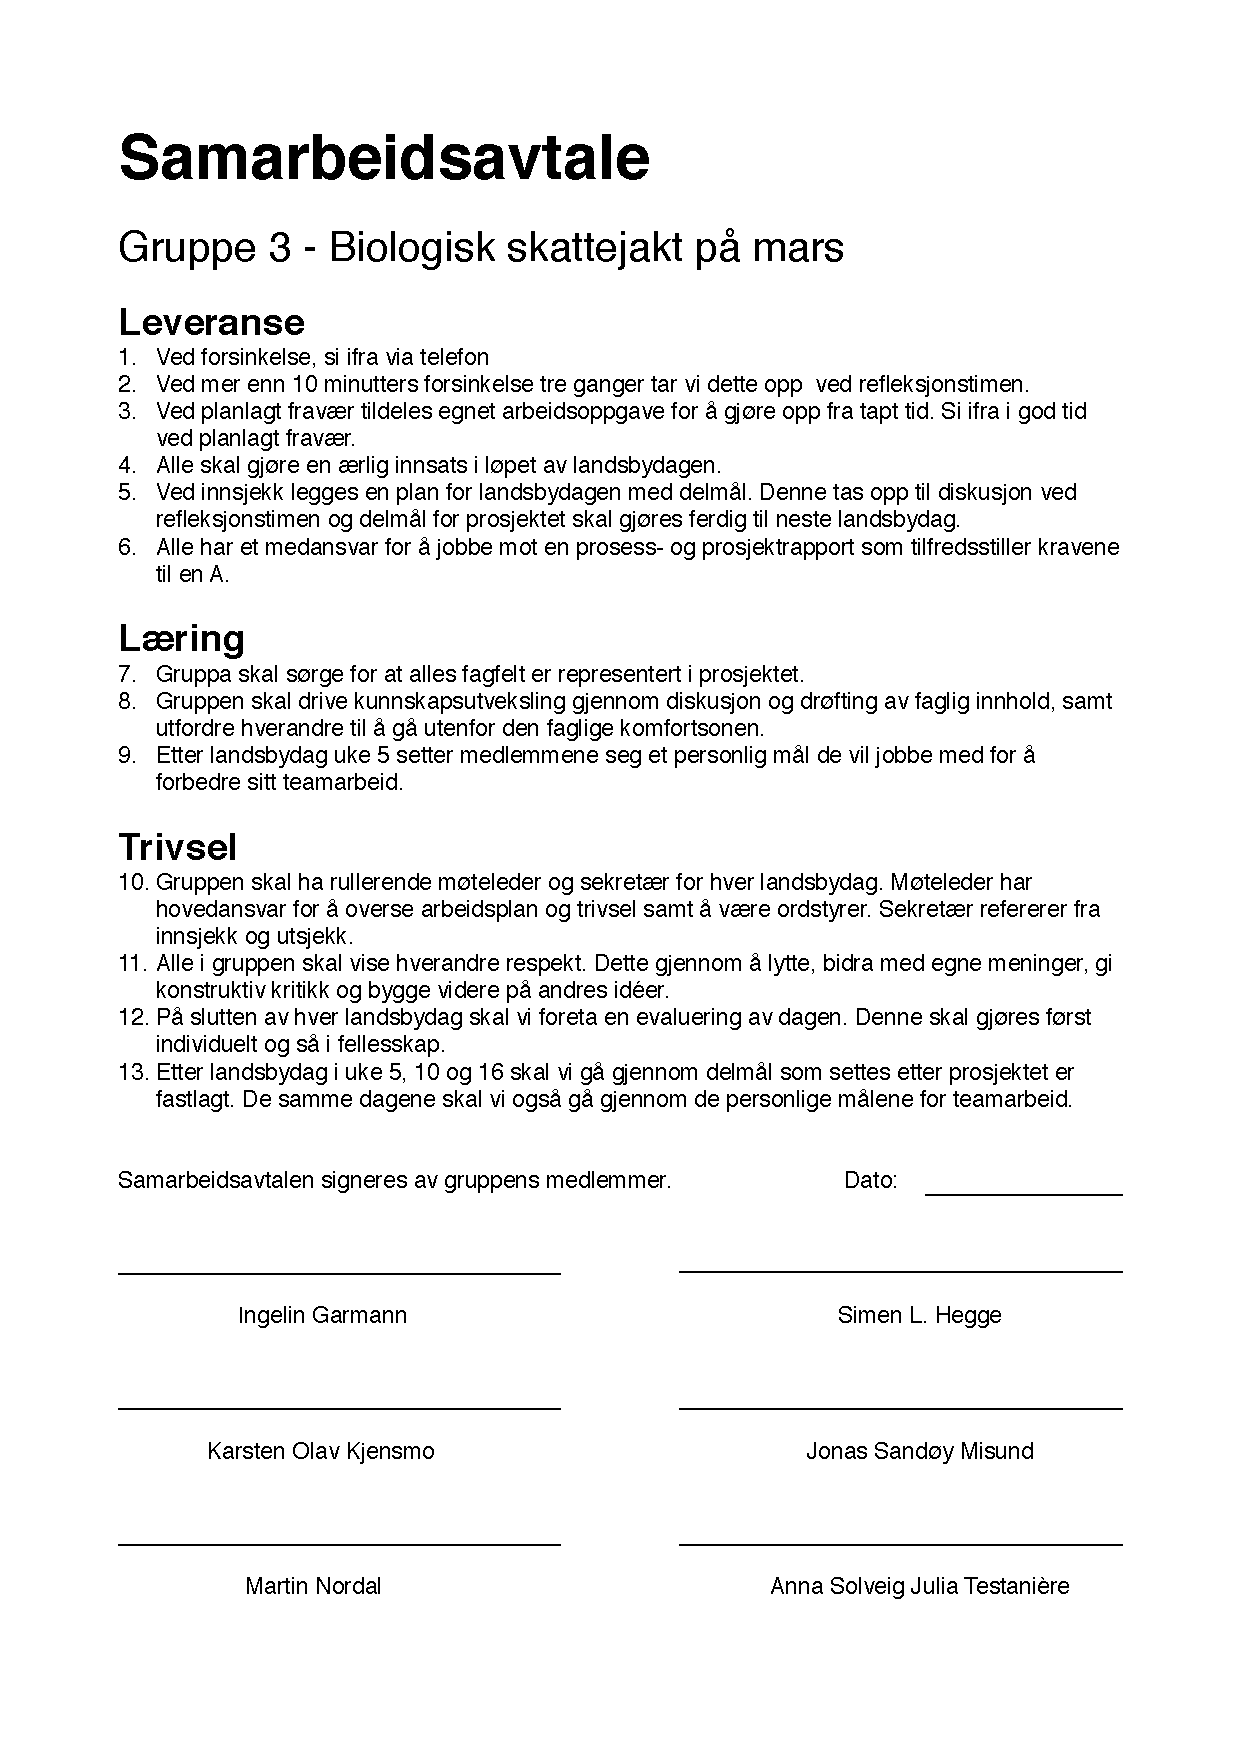
\includegraphics[width=0.9\textwidth]{Samarbeidsavtale_2.pdf}
\end{center}

\end{appendices}

\end{document}